\hypertarget{introduction}{%
\section{Introduction}\label{introduction}}

\hypertarget{model-and-methods}{%
\section{Model and Methods}\label{model-and-methods}}

We first develop the infinitesimal model (in the sense of
{[}@barton2017{]}, i.e.~the `Gaussian descendants' approximation
{[}@turelli2017{]}) for an autotetraploid population. We then consider
mixed-ploidy populations in which diploids, triploids and tetraploids
coexist and interbreed through the production of haploid and diploid
gametes that combine freely.

\hypertarget{the-infinitesimal-model}{%
\subsection{The infinitesimal model}\label{the-infinitesimal-model}}

Consider a population which expresses a quantitative trait determined by
a large number of additive loci of small effect. The infinitesimal model
approximates the inheritance of such a trait by assuming that the trait
value \(Z_{ij}\) of a random offspring from parents with trait values
\(z_i\) and \(z_j\) follows a Gaussian distribution with mean equal to
the midparent value and variance which is independent of the mean:
\begin{align}
  Z_{ij} \sim \Normal\left(\frac{z_i + z_j}{2}, V_{ij}\right)
  \label{eq:inf}
  \end{align} Here, \(V_{ij}\) is referred to as the \emph{segregation
variance} in family \((i,j)\). This is the variation generated among
offspring from the same parental pair due to random Mendelian
segregation in meiosis. This approximation can be justified as arising
from the limit where the number of loci determining the trait tends to
infinity {[}@barton2017{]}. An alternative, and for our purposes useful,
way to characterize the model in diploids and polyploids is to write
\(Z_{ij} = Y_i + Y_j\), where \(Y_i\) and \(Y_j\) are independent
Gaussian random variables
\(Y_i \sim \Normal\left(\frac{z_i}{2}, V_i\right)\) (and similarly for
\(Y_j\)). We refer to \(Y_i\) as the (random) gametic value of
individual \(i\), and to \(V_i\) as the \emph{gametic segregation
variance} of individual \(i\). This formulation is helpful in that it
highlights that Mendelian segregation occurs independently in both
parents when gametes are produced, which then combine additively to
determine the offspring trait value.

If we assume a population consisting of infinitely many unrelated
individuals, expressing a trait with genetic variance \(V\) and
segregation variance \(V_0\), we find that under random mating the
variance in the offspring generation is \begin{align}
V' &= \Ex[\Var[Z_{ij}|Z_i, Z_j]] + \Var[\Ex[Z_{ij}|Z_i,Z_j]] \nonumber \\
   &= \Ex[V_{ij}] + \Var\left(\frac{Z_i + Z_j}{2}\right) \nonumber \\
   &= V_0 + \frac{V}{2}\ .
   \label{eq:eq}
\end{align} So that at equilibrium (\(V'=V\)), we have \(V = 2V_0\)
{[}@barton2017{]}. If we denote by \(X\) the contribution to the trait
value associated with a randomly sampled haploid genome from the
population, we also have that, at equilibrium, \(V=2V_0=mV_x\), where
\(V_x = \Var[X]\). Note that no assumptions regarding ploidy level have
been made in the definition of the model. Indeed, as long as all
individuals are of the same \emph{even} ploidy level, eq.~\ref{eq:inf}
and eq.~\ref{eq:eq} apply equally well to the inheritance of an additive
trait in polyploids as in diploids. Two factors however do lead to
differences with the standard diploid model due to their effect on
\(V_i\): (1) the potential occurrence of double reduction in polyploids
affects the relationship between \(V_x\) and \(V_0\) and (2) the
evolution of the segregation variance over time in finite populations is
affected by the ploidy level.

\hypertarget{the-effect-of-double-reduction-on-the-segregation-variance}{%
\subsection{The effect of double reduction on the segregation
variance}\label{the-effect-of-double-reduction-on-the-segregation-variance}}

When an autotetraploid forms quadrivalents during prophase I, a form of
`internal inbreeding' may occur as a result of the phenomenon called
\emph{double reduction} {[}@lynch1998 p.~57{]}. Double reduction happens
when, as a result of recombination, replicated gene copies on sister
chromatids move to the same pole during anaphase I, as illustrated in
fig.~\ref{fig:dr}. In the example shown in fig.~\ref{fig:dr}, one of the
four generated gametes is \(AA\), which would not occur in the ordinary
bivalent meiosis, because in that case, paired chromosomes (involved in
cross-overs) are separated during anaphase I. The frequency of double
reduction at a locus in the presence of multivalent formation is hence
determined by the frequency at which that locus is involved in a
cross-over (which depends on the distance to the centromere), and has an
upper bound at \(1/6\) {[}@stift2008{]}.

When double reduction occurs, an \(ABCD\) genotype would generate 10
distinct gametes, as opposed to 6 in when chromosomes form bivalents. As
a result, the segregation variance is increased by double reduction. 
For
a random genotype \(X_1X_2X_3X_4\), we can find the gametic segregation
variance contributed by a locus when double reduction happens as
\begin{align*}
    \Ex[\var[Y|X_1,X_2,X_3,X_4]] &= \var[Y] - \Var[\Ex[Y|X_1,X_2,X_3,X_4]] \\
        &= \var[2X] - \var\left[\frac1 4 (2X_1 + 2X_2 + 2X_3 + 2X_4)\right] \\
        &= 4v_x - \frac{1}{4}4v_x 
        = 3v_x
\end{align*} where \(X\) denotes the additive effect of a random allele
at the locus drawn from the reference population and \(v_x = \Var[X]\).
In the absence of double reduction we have \begin{align*}
    \Ex[\var[Y|X_1,X_2,X_3,X_4]] 
        &= 2\Var[X] - \var\left[\frac1 6 \sum_{i=1}^3 \sum_{j=i+1}^4(X_i+X_j)\right]
        = v_x
\end{align*} Assuming that the probability of double reduction at any
locus is \(\alpha\) (also \(\alpha_4\) below), and summing over
independent loci, we find that the gametic segregation variance in the
presence of double reduction should be \begin{equation}
\frac{V_0}{2} = (1-\alpha)V_x + 3\alpha V_x = V_x(1+2\alpha).
\label{eq:dr}
\end{equation}

\begin{figure}
\begin{center}
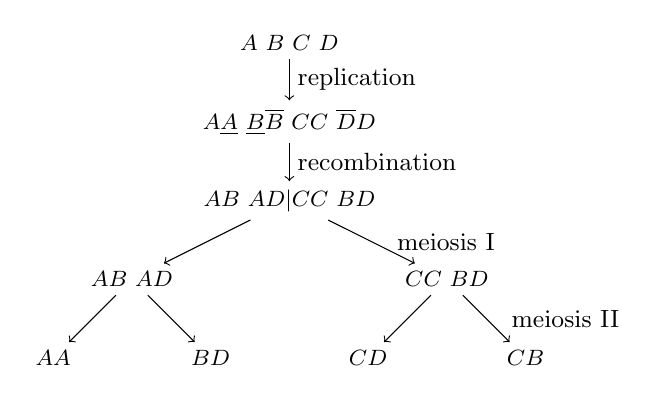
\begin{tikzpicture}
\footnotesize
\node (n1) at (0, 5) [] {$A\ B\ C\ D$};
\node (n2) at (0, 4) [] {$A\underline{A}\ \underline{B}\overline{B}\ CC\ \overline{D}D$};
\node (n3) at (0, 3) [] {$AB\ AD | CC\ BD$};
\node (n4) at (-2, 2) [] {$AB\ AD$};
\node (n5) at ( 2, 2) [] {$CC\ BD$};
\node (n6) at (-3, 1) [] {$AA$};
\node (n7) at (-1, 1) [] {$BD$};
\node (n8) at ( 3, 1) [] {$CB$};
\node (n9) at ( 1, 1) [] {$CD$};
\draw[->] (n1) -- (n2) node [right,midway] {\small replication};
\draw[->] (n2) -- (n3) node [right,midway] {\small recombination};
\draw[->] (n3) -- (n4);
\draw[->] (n3) -- (n5) node [right,midway] {\small \ \ meiosis I};
\draw[->] (n5) -- (n8) node [right,midway] {\small \ \ meiosis II};
\draw[->] (n5) -- (n9);
\draw[->] (n4) -- (n6);
\draw[->] (n4) -- (n7);
\end{tikzpicture}
\end{center}
\begin{caption}{
Schematic illustration of a meiotic division in an autotetraploid leading to
double reduction at a locus with genotype $ABCD$.
Two recombination events are assumed to occur at the locus (denoted by the
bars).
\label{fig:dr}
}\end{caption}
\end{figure}

\hypertarget{inbreeding-in-autotetraploids}{%
\subsection{Inbreeding in
autotetraploids}\label{inbreeding-in-autotetraploids}}

In a finite population the segregation variance will decrease over time
due to inbreeding. Indeed, in a diploid individual for instance, when
the two gene copies at a locus are identical, segregation will not
generate any variation. The rate of inbreeding depends on the ploidy
level {[}@moody1993; @arnold2012{]}, and hence the rate at which the
segregation variance declines \emph{does} so too. Let \(F_i\) the
inbreeding coefficient of individual \(i\), defined as the probability
that two \emph{distinct} gene copies at a locus in individual \(i\) are
identical by descent (IBD) with respect to some reference population,
and let \(\Phi_{ij}\) be the coancestry coefficient for individuals
\(i\) and \(j\), defined as the probability that two genes sampled
independently from \(i\) and \(j\) at a given locus are IBD. In
diploids, one can show that the gametic segregation variance \(V_i\) is
decreased by a factor \(1-F_i\) relative to the segregation variance in
the reference population \(V_0/2\) {[}@barton2017{]}. In polyploids,
however, \(F_i\) does not suffice to describe the state of homozygosity
in individual \(i\). In tetraploids, for instance, we have five distinct
homozygosity states, which we can symbolically represent as
\(abcd, aabc, aabb, aaab\) and \(aaaa\) (in general, the number of
homozygosity states grows according to the partition function
\((1,2,3,5,7,11,15,22,\dots)\)). Representing the probability of being
in these five increasingly homozygous states as
\(\delta_1, \dots, \delta_5\), we find that the gametic segregation
variance is reduced by a factor
\[\phi = \delta_1 + \left(1 - \frac1 6\right) \delta_2 + \left(1 - \frac1
        3\right)\delta_3 + \left(1 - \frac1 2\right) \delta_4\] which is
precisely \(1-F_i\), as in diploids (see also {[}@moody1993{]}). This
shows that we do not need to track the array of homozygosity
coefficients in order to compute the segregation variance in a
tetraploid family, but only require the inbreeding coefficients of the
parents. This is a consequence of the fact that, in tetraploids, gametes
are diploid. For higher ploidy levels, one would need to track higher
order identity coefficients. We shall hence not consider higher ploidy
levels in this paper.

In order to efficiently conduct individual-based simulations under the
infinitesimal model, we hence need to be able to track the \(F_i\) and
\(\Phi_{ij}\). Denoting the parents of individual \(i\) by \(k\) and
\(l\), the recursion for the inbreeding coefficients is \begin{align}
    F_i &= \Phi_{kl}& \text{in diploids} \nonumber \\  
    F_i &= \frac1 6 (F_k^\ast + F_l^\ast + 4\Phi_{kl}) & \text{in tetraploids} 
    \label{eq:recursion}
\end{align} where \(F_k^\ast = \alpha + (1-\alpha)F_k\). The recursion
for the tetraploid case follows from considering three cases: either (1)
the two genes sampled in individual \(i\) both came from the gamete
contributed by parent \(k\), which happens with probability \(1/6\), in
which case they are IBD with probability \(F_k^\ast\); or (2) as in (1)
but from parent \(l\); or (3) with probability \(2/3\) the two genes
came from different gametes, in which case they are IBD with probability
\(\Phi_{kl}\). The recursion for the coancestry coefficients in
\(m\)-ploids is given by \begin{align}
    \Phi_{ii} &= \frac1 m \left(1 + (m-1)F_i\right) \nonumber \\
    \Phi_{ij} &= \sum_k \sum_l P_{ik}P_{jl} \Phi_{kl} & i \ne j 
    \label{eq:coancestry}
\end{align} where the sums are over individuals in the parental
population, and where \(P_{ik} \in \{0, \frac1 2, 1\}\) is the
probability that a gene copy in \(i\) is derived from parent \(k\). When
dealing with discrete generations, \(P_{ik}\) values can be conveniently
represented in a \(N(t) \times N(t-1)\) matrix, where \(N(t)\) is the
population size in generation \(t\), so that
\(\Phi(t) = P \Phi(t-1) P^T\), where \(\Phi(t)\) is the matrix of
coancestry coefficients in generation \(t\) {[}@barton2017{]}.

\hypertarget{the-infinitesimal-model-in-mixed-ploidy-populations}{%
\subsection{The infinitesimal model in mixed-ploidy
populations}\label{the-infinitesimal-model-in-mixed-ploidy-populations}}

When considering mixed-ploidy populations, we need to consider how
equilibrium variances in the model scale with ploidy level, and how
offspring of different ploidy levels are derived from a parental pair.
Throughout the following paragraphs, we specialize to a
diploid-triploid-tetraploid complex. A glossary of the relevant notation
can be found in tbl.~\ref{tbl:glossary}.

\hypertarget{scaling-of-the-genetic-variance-across-ploidy-levels}{%
\subsubsection{Scaling of the genetic variance across ploidy
levels}\label{scaling-of-the-genetic-variance-across-ploidy-levels}}

The equilibrium phenotypic variance \(V\) under the infinitesimal model
was derived above as \(2V_0\), where \(V_0\) is the segregation variance
(eq.~\ref{eq:eq}). As noted below eq.~\ref{eq:eq}, this entails that for
\(m\)-ploids, \(2V_0 = mV_{x,m}\), where \(V_{x,m}\) is the variance of
the additive effect of a randomly sampled haploid genome from the
reference \(m\)-ploid population. Now, in a mixed-ploidy system, it is
not immediately clear how the \(V_{x,m}\) should scale across ploidy
levels, as this depends on the effects of polyploidization \emph{per se}
on additive allelic effects {[}@porturas2019; @clo2021; @clo2022{]}. If
we assume equal equilibrium variances (and concomitantly segregation
variances), the genetic variance for a haploid genome in tetraploids
will be half that of diploids, entailing a reduction in the additive
allelic effect per locus as ploidy level rises. On the other hand, if we
assume equal allelic effects, and hence that the genetic variance
associated with a hypothetical haploid genome copy is identical across
ploidy levels, then the segregation and equilibrium variances in
tetraploids will be twice those of diploids, and the associated
phenotypic range will be doubled as well.

To ease interpretation, let us consider an underlying Mendelian system,
consisting of \(n\) unlinked additive bi-allelic loci in Hardy-Weinberg
and linkage equilibrium (HWLE). Assuming that the additive effects in
tetraploids are homogeneously scaled by a factor \(\beta\) relative to
those in diploids, and writing \(V_{z,m}\), \(V_{0,m}\) and \(V_{x,m}\)
for respectively the equilibrium genetic variance, the segregation
variance and the genetic variance associated with a haploid genome in
\(m\)-ploids, the following relationships hold: \[
 \frac{V_{z,4}}{V_{z,2}} = \frac{2V_{0,4}}{2V_{0,2}} = \frac{4V_{x,4}}{2V_{x,2}} =
 \frac{2 \sum_i^n (\beta a_i)^2 p_i(1-p_i)}{\sum_i^n a_i^2 p_i(1-p_i)} =
 2\beta^2
\] So we see that assuming equal equilibrium phenotypic variances
\(V_{z,4}/V_{z,2} = 1\) entails that allelic effects are scaled by a
factor \(\beta=\sqrt{1/2}\). On the other hand, assuming equal allelic
effects (\(\beta=1\)) entails that the phenotypic variance at
equilibrium in tetraploids is twice that of diploids, as we noted above.
To study the effect of such assumptions, we introduce \(\beta_m\) as a
parameter so that \(V_{z,m} = \frac{m}{2}\beta_m^2 V_{z,2}\), keeping in
mind its interpretation as a scaler of allelic effects in the underlying
Mendelian system, and setting \(\beta_2=1\). The trait value
distribution for offspring of ploidy level \(m_{ij}\) from parental pair
\((i,j)\) with ploidy levels \(m_i\) and \(m_j\), formed through the
union of a \(g_i\)-ploid gamete from parent \(i\) and a \(g_j\)-ploid
gamete from parent \(j\) will then be \[Z_{ij} \sim \Normal\left(
    \beta_{m_{ij}} \left(
          \frac{g_i}{m_i}\frac{z_i}{\beta_{m_i}} 
        + \frac{g_j}{m_j}\frac{z_j}{\beta_{m_j}}\right), V_{i,g_i} + V_{j,g_j}\right)\]
Where \(V_{i,g_i}\) is the gametic segregation variance associated with
the formation of a \(g_i\)-ploid gamete by individual \(i\). We now
proceed to characterize the \(V_{i,g_i}\) and their evolution over time.

\hypertarget{unreduced-gamete-formation-in-diploids}{%
\subsubsection{Unreduced gamete formation in
diploids}\label{unreduced-gamete-formation-in-diploids}}

\begin{figure}
\begin{center}
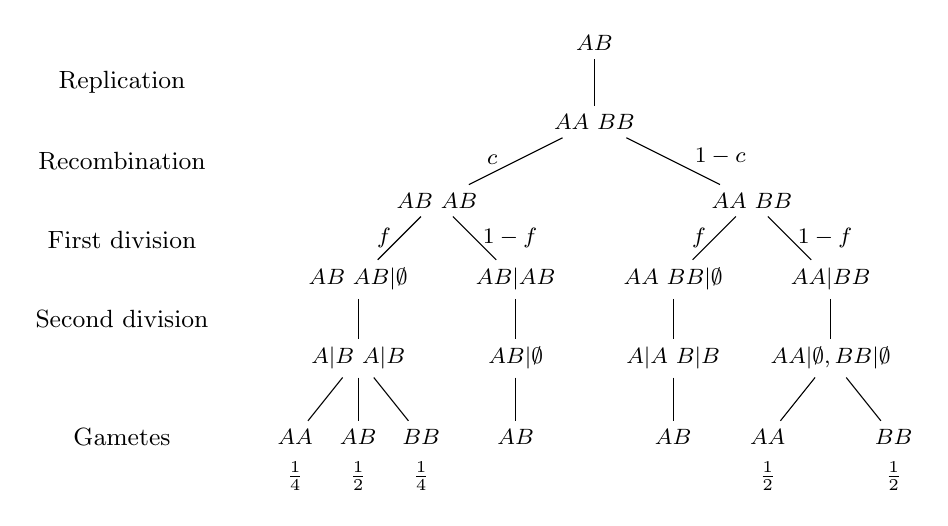
\begin{tikzpicture}
\footnotesize
\node (rep) at (-6, 4.5) [] {\small Replication};
\node (rep) at (-6, 3.5) [] {\small Recombination};
\node (rep) at (-6, 2.5) [] {\small First division};
\node (rep) at (-6, 1.5) [] {\small Second division};
\node (rep) at (-6, 0)   [] {\small Gametes};
\node (Aa)  at (0, 5) [] {$AB$};
\node (AAaa)  at (0, 4) [] {$AA\ BB$};
\node (rAaAa) at (-2, 3) [] {$AB\ AB$};
\node (rAAaa) at ( 2, 3) [] {$AA\ BB$};
\path (Aa) edge (AAaa);
\path (AAaa) edge node[near end, above] {$c$} (rAaAa) ;
\path (AAaa) edge node[near end, above] {\qquad $1-c$} (rAAaa);

\node (fdr11) at (-3, 2) [] {$AB\ AB | \emptyset$};
\node (fdr12) at (-3, 1) [] {$A|B\  A|B$}; 
\node (AA) at (-3.8,0) [] {$AA$};
\node (p1) at (-3.8,-0.5) [] {$\frac{1}{4}$};
\node (Aa) at (-3,0) [] {$AB$};
\node (p2) at (-3,-0.5) [] {$\frac{1}{2}$};
\node (aa) at (-2.2,0) [] {$BB$};
\node (p2) at (-2.2,-0.5) [] {$\frac{1}{4}$};
\path (fdr12) edge (AA);
\path (fdr12) edge (Aa);
\path (fdr12) edge (aa);
\path (fdr11) edge (fdr12);
\path (rAaAa) edge node[left] {$f$} (fdr11);

\node (sdr11) at (-1, 2) [] {$AB | AB$}; 
\node (sdr12) at (-1, 1) [] {$AB | \emptyset$}; 
\node (Aa2) at (-1,0) [] {$AB$};
\path (sdr12) edge (Aa2);
\path (sdr11) edge (sdr12);
\path (rAaAa) edge node[right] {$1-f$} (sdr11);

\node (fdr21) at (1,2) [] {$AA\ BB|\emptyset$};
\node (fdr22) at (1,1) [] {$A|A\ B|B$};
\node (Aa3) at (1,0) [] {$AB$};
\path (rAAaa) edge node[left] {$f$} (fdr21);
\path (fdr21) edge (fdr22);
\path (fdr22) edge (Aa3);

\node (sdr21) at (3, 2) [] {$AA | BB$};
\node (sdr22) at (3, 1) [] {$AA| \emptyset, BB|\emptyset$};
\node (AA4) at (2.2,0) [] {$AA$};
\node (p1) at (2.2, -0.5) [] {$\frac{1}{2}$};
\node (aa4) at (3.8,0) [] {$BB$};
\node (p2) at (3.8, -0.5) [] {$\frac{1}{2}$};
\path (rAAaa) edge node[right] {$1-f$} (sdr21);
\path (sdr21) edge (sdr22);
\path (sdr22) edge (AA4);
\path (sdr22) edge (aa4);
\end{tikzpicture}
\begin{caption}{
Schematic representation of the different pathways for unreduced gamete
formation in diploids and their different outcomes.
\label{fig:udip}
}\end{caption}
\end{center}
\end{figure}

The mechanisms of unreduced gamete formation do not necessarily lead to
a faithful transmission of the complete diploid genome. Unreduced
gametes are formed in two ways, depending on the meiotic abberation that
leads to their origin: (1) first division restitution (FDR) of (2)
second division restitution (SDR) {[}@bretagnolle1995{]}. Consider a
locus in a diploid with two distinct genes \(A\) and \(a\). Assume
recombination happens with probability \(c\) and that conditional on
unreduced gamete formation, formation is due to FDR with probability
\(f\) while it is due to SDR with probability \(1-f\). The different
unreduced gametes that are formed are represented schematically in
fig.~\ref{fig:udip}. Writing the genotype at a locus in the diploid
parent as \(X_1X_2\), with allelic effects \(X_1\) and \(X_2\), the
genotypic value of an unreduced gamete at this locus will be
\[Y = \begin{cases}
    2X_1 & \text{w.p. } \alpha_2/2 = \frac1 4 f c + \frac1 2 (1-f)(1-c) \\
    2X_2 & \text{w.p. } \alpha_2/2 \\
    X_1 + X_2 & \text{w.p. } 1-\alpha_2 
    \end{cases}\] where \(\alpha_2 = 1 - f - c + \frac{3}{2}cf\) is the
probability that two copies of the same gene end up in a diploid gamete
produced by a diploid individual. Conditional on the latter event, we
get, by a similar reasoning as the one leading eq.~\ref{eq:dr}, a
segregation variance equal to \begin{align*}
\Ex[\Var[Y|X_1,X_2]] &= \Var[Y] - \Var[\Ex[Y|X_1,X_2]] \\
    &= \Var[2X] - \Var\left[\frac{1}{2}(2X_1 + 2X_2)\right] \\
    &= 2v_x
\end{align*} Conditioning on the complementary event, all gametes have
genetic value \(Y = X_1+X_2\), so that the segregation variance is 0.
Summing across independent loci, we have
\(V_{i,2} = 2\alpha_2(1-F_i)V_x\) for a diploid individual \(i\).

\hypertarget{meiosis-in-triploids}{%
\subsubsection{Meiosis in triploids}\label{meiosis-in-triploids}}

Triploids, when viable, may be important for the dynamics of
mixed-ploidy populations due to the formation of a so-called triploid
bridge. The formation of triploids presents no immediate issues, we
simply need to track the segregation variance contributions from both
donor gametes, and relate these to \(V_{0,3}\). Sexual reproduction in
triploids is however more complicated. There are no known mechanisms to
coordinate the assortment of chromosomes in for instance a haploid and
diploid gamete, and meiosis, if it happens, usually results in aneuploid
gametes {[}@ramsey1998{]}. Experimental results indicate that, at least
in yeast, triploids usually form trivalents and undergo recombination,
after which each trivalent is randomly assorted in the daughter cells,
some receiving one, others two copies of a given chromosome
{[}@charles2010{]}. In the absence of gametic nonreduction, the
probability of obtaining euploid gametes (two diploid and two haploid
gametes) from such a process is \((1/2)^n\), where \(n\) is the number
of chromosomes. If the number of chromosomes is small this is not
negligible, for instance in \emph{A. thaliana} we would have
\((1/2)^5 \approx 0.03\), which is of the same order as the unreduced
gamete formation rate. Unreduced (triploid) gametes may also be produced
and important for the dynamics of mixed-ploidy populations
{[}@ramsey1998{]}. However, they generate additional difficulty, since
in order to compute the contributed variance under inbreeding, we would
need an additional identity coefficient recording the probability that
three genes are IBD at a locus. We will hence ignore the possibility of
unreduced gamete production in triploids. Denoting by \(\alpha_3\) the
probability that a diploid gamete produced by a triploid individual
contains two copies of the same parental gene, we can use the same
approach as above to derive \(V_{i,1}\) and \(V_{i,2}\) for a triploid
individual \(i\). We note that, on the supposition that diploid gametes
are produced by random assortment of chromosomes in a haploid and
diploid gametes, \(\alpha_3 \le 1/4\). The formulae for the different
\(V_{i,g_i}\) are summarized in tbl.~\ref{tbl:segvar}.

\begin{longtable}[]{@{}
  >{\raggedright\arraybackslash}p{(\columnwidth - 4\tabcolsep) * \real{0.2857}}
  >{\centering\arraybackslash}p{(\columnwidth - 4\tabcolsep) * \real{0.3571}}
  >{\raggedleft\arraybackslash}p{(\columnwidth - 4\tabcolsep) * \real{0.3571}}@{}}
\caption{Gametic segregation variance for different cytotype \(\times\)
gametic cytotype combinations. \(V_x\) refers to genetic variance
associated with a haploid genome in the reference population of the
cytotype to which the gamete will contribute. Under the assumptions
outlined in the main text, we have the following constraints for the
\(\alpha_k\): \(\alpha_2 \le 1\), \(\alpha_3 \le 1/4\) and
\(\alpha_4 \le 1/6\). \label{tbl:segvar}}\tabularnewline
\toprule()
\begin{minipage}[b]{\linewidth}\raggedright
\textbf{cytotype}
\end{minipage} & \begin{minipage}[b]{\linewidth}\centering
\(V_{i,1}\) (haploid)
\end{minipage} & \begin{minipage}[b]{\linewidth}\raggedleft
\(V_{i,2}\) (diploid)
\end{minipage} \\
\midrule()
\endfirsthead
\toprule()
\begin{minipage}[b]{\linewidth}\raggedright
\textbf{cytotype}
\end{minipage} & \begin{minipage}[b]{\linewidth}\centering
\(V_{i,1}\) (haploid)
\end{minipage} & \begin{minipage}[b]{\linewidth}\raggedleft
\(V_{i,2}\) (diploid)
\end{minipage} \\
\midrule()
\endhead
diploid \((m_i = 2)\) & \(\frac{1}{2}(1-F_i)V_x\) &
\(2\alpha_2 (1-F_i)V_x\) \\
triploid \((m_i = 3)\) & \(\frac{2}{3}(1-F_i)V_x\) &
\(\frac{2}{3}(1 + 3\alpha_3)(1-F_i)V_x\) \\
tetraploid \((m_i = 4)\) & -- & \((1+2\alpha_4)(1-F_i)V_x\) \\
\bottomrule()
\end{longtable}

\hypertarget{recursions-for-inbreeding-coefficients}{%
\subsubsection{Recursions for inbreeding
coefficients}\label{recursions-for-inbreeding-coefficients}}

In a mixed-ploidy system tracking inbreeding coefficients becomes only
slightly more complicated. Recall that \(\alpha_m\) is the probability
that a diploid gamete from an \(m\)-ploid individual transmits two
copies of the same gene at some locus. Let \(m_i\) denote the ploidy
level of individual \(i\). We still have the recursion shown in
eq.~\ref{eq:recursion}, where now
\[F_k^\ast = F_k(1-\alpha_{m_k}) + \alpha_{m_k}\] For a triploid
individual, where the parent contributing the \(2n\) gamete is \(k\), we
have \[ F_i = \frac1 3 \left(F_k^\ast + 2\Phi_{kl}\right) \] For
\(\Phi\) the recursion in eq.~\ref{eq:coancestry} remains valid, but
where diagonal elements are now given by
\[\Phi_{ii} = \frac{1}{m_i} \left(1 + (m_i-1)F_i\right)\] and where the
elements of the the pedigree matrix \(P\) now have entries in
\(\{0,\frac1 3,\frac1 2,\frac2 3,1\}\).

\hypertarget{population-dynamics}{%
\subsubsection{Population dynamics}\label{population-dynamics}}

\emph{What comes here depends on the results we will include.}

The dynamics of the mixed-ploidy system (in the absence of selection on
the trait) are determined by the rates at which different types of
gametes are formed. We assume an individual of ploidy level \(k\) forms
haploid and diploid gametes with proportions \(u_{k1}\) and \(u_{k2}\),
so that the (relative) fecundity of a \(k\)-ploid individual is
\(u_{k1} + u_{k2}\). Unless stated otherwise, we will assume \[U = 
    \begin{pmatrix} 
    u_{21} & u_{22} \\ 
    u_{31} & u_{32} \\ 
    u_{41} & u_{42} 
    \end{pmatrix} =
    \begin{pmatrix} 
    1-u & u \\
    v & v \\
    0 & 1-u
    \end{pmatrix}\] where \(u\) is referred to as the proportion of
unreduced gametes, and \(2v\) is the proportion of euploid gametes
produced by a triploid individual. An analysis of a deterministic model
for the cytotype dynamics {[}also analyzed in@felber1991; @felber1997{]}
is included in sec.~\ref{sec:det}.

\hypertarget{tbl:glossary}{}
\begin{longtable}[]{@{}
  >{\raggedright\arraybackslash}p{(\columnwidth - 2\tabcolsep) * \real{0.0870}}
  >{\raggedright\arraybackslash}p{(\columnwidth - 2\tabcolsep) * \real{0.9130}}@{}}
\caption{\label{tbl:glossary}Glossary for the notation used to define
the mixed-ploidy infinitesimal model.}\tabularnewline
\toprule()
\begin{minipage}[b]{\linewidth}\raggedright
Symbol
\end{minipage} & \begin{minipage}[b]{\linewidth}\raggedright
Explanation
\end{minipage} \\
\midrule()
\endfirsthead
\toprule()
\begin{minipage}[b]{\linewidth}\raggedright
Symbol
\end{minipage} & \begin{minipage}[b]{\linewidth}\raggedright
Explanation
\end{minipage} \\
\midrule()
\endhead
\(z_i\) & Trait value of individual \(i\) \\
\(Z_{ij}\) & Trait value of a random offspring from parental pair
\((i,j)\) \\
\(V_{z,m}\) & Equilibrium variance in an \(m\)-ploid population \\
\(V_{0,m}\) & Segregation variance in the \(m\)-ploid reference
population \\
\(V_{x,m}\) & Equilibrium variance of a haploid genome in the
\(m\)-ploid reference population \\
\(V_{i,m}\) & Gametic segregation variance in individual \(i\) \\
\(F_i\) & Inbreeding coefficient of individual \(i\) \\
\(\Phi_{ij}\) & Coancestry coefficient of individuals \(i\) and \(j\) \\
\(m_i\) & Ploidy level of individual \(i\) \\
\(\alpha_m\) & Probability that a diploid gamete from an \(m\)-ploid
individual contains two copies of the same parental gene \\
\(\beta_m\) & Scaling factor for the allelic effects in ploidy level
\(m\) \\
\(u_{m,g}\) & Proportion of \(g\)-ploid gametes produced by an
\(m\)-ploid individual \\
\(u\) & Proportion of unreduced gametes in even-ploids \\
\(v\) & Proportion of haploid and diploid gametes in triploids \\
\bottomrule()
\end{longtable}

\hypertarget{results}{%
\section{Results}\label{results}}

We first verify that, in the absence of inbreeding, our implementation
of the mixed-ploidy infinitesimal model yields the predicted equilibrium
variance for each cytotype (fig.~\ref{fig:z}) and the expected
equilibrium proportions (fig.~\ref{fig:eqp}). We next evaluate the
accuracy of the infinitesimal model as an approximation to the evolution
of a quantitative trait determined by \(L\) additive loci. We find that
the infinitesimal model with inbreeding generally yields accurate
predictions for the evolution of the genetic variance, even as the
number of loci becomes fairly small (e.g.~\(L=50\), fig.~\ref{fig:vz}).
For \(L=20\), substantial deviations from the infinitesimal
approximation can be observed, although it may still be considered
reasonable (fig.~\ref{fig:vz}).

Although inbreeding is slower in autotetraploids than in diploids for
the same population size, the tetraploid fraction of a diploid-dominated
mixed-ploidy population will have an equal or higher average inbreeding
coefficient (fig.~\ref{fig:f1}). This is because in such a population,
triploid and tetraploid individuals mostly arise from gametes formed by
diploid individuals or polyploid individuals with very recent diploid
ancestry (about \(1+u+2v\) generations ago for tetraploids, and
\(1+\frac{2}{3}(u+2v)\) generations ago for triploids, see
sec.~\ref{sec:ttdip}), so that the polyploid subpopulations will show an
average relatedness similar to the diploid population and not evolve as
an isolated higher-ploidy population would. A nonzero probability of
producing IBD diploid gametes (\(\alpha\)) will then further increase
the inbreeding coefficient in the tetraploid and triploid fraction of
the population relative to their diploid progenitors
(fig.~\ref{fig:f1}). Therefore, as long as diploids dominate, the effect
of harboring some of the gene pool in triploid and tetraploid
individuals on the rate of inbreeding is negligible, and we find that
the evolution of the inbreeding coefficient over time is well predicted
by \(1-e^{-t/2N_e}\), where the inbreeding-effective population size is,
to first order in \(u\), given by \((1-2u)N\) (sec.~\ref{sec:effsize},
fig.~\ref{fig:fNe}).

\hypertarget{discussion}{%
\section{Discussion}\label{discussion}}

\begin{itemize}
\item
  It appears that many papers on diploid -- tetraploid contact zones or
  mixed-ploidy populations fail to find significant numbers of
  triploids. Note though that such studies focus on established
  tetraploids, where the cytotypes may have diverged to some extent,
  whereas we focus on the case where a tetraploid cytotype has not yet
  established. The model is therefore more relevant for populations that
  are likely to be referred to as diploid. It remains to be seen to what
  extent such populations actually exhibit a mixed-ploidy equilibrium.
  See {[}@suda2013{]} and {[}@herben2016{]}.
\item
  The issue with dominance. On the one hand, it is often said that
  polyploids accumulate a larger mutation load, and will hence show
  inbreeding depression, but this really only applies to already
  established polyploid populations. Similarly, the sort of effects of
  dominancestudied in Booker and Schrider during range expansions apply
  mostly to polyploids that have accumulated a large mutation load over
  a rather long time as a stable polyploid population. In our case,
  polyploids are virtually always derived very recently from diploid
  ancestors, so they will not have accumulated more deleterious
  recessives than their diploid counterparts. As inbreeding will be
  slower in tetraploids, we should hence have reduced inbreeding
  expression, as we have the same load as in diploids, but it is less
  expressed (at least when considering recessives). There should
  therefore be an immediate benefit to polyploidy (reduced inbreeding
  depression), which is however a long term disadvantagem because
  eventually the established polyploid will start to accumulate a higher
  load due to less efficient purging.
\end{itemize}

\hypertarget{references}{%
\section{References}\label{references}}

\hypertarget{refs}{}
\begin{CSLReferences}{0}{0}
\end{CSLReferences}

\clearpage
\setcounter{page}{1}

\clearpage
\renewcommand{\thefigure}{S\arabic{figure}}
\renewcommand{\thesection}{S\arabic{section}}
\renewcommand{\theequation}{S\arabic{equation}}
\renewcommand{\thealgorithm}{S\arabic{algorithm}}
\setcounter{figure}{0}
\setcounter{section}{0}
\setcounter{equation}{0}
\setcounter{algorithm}{0}

\hypertarget{supplementary-figures}{%
\section{Supplementary figures}\label{supplementary-figures}}

\clearpage

\begin{figure}
\hypertarget{fig:z}{%
\centering
\includegraphics{/home/arthur_z/vimwiki/build/img/2023-10-10/mixedploidy-eq.svg}
\caption{Equilibrium trait value (\(z\)) distribution in a mixed-ploidy
population evolving according to the infinitesimal model without
inbreeding for three different scaling assumptions of allelic effects
across ploidy levels. Histograms (lines) show simulation results,
whereas the filled Gaussian densities show the expected distribution at
equilibrium \(\Normal\left(0, k\beta_k^2V_x\right)\). In the
\(\beta=(1,1,1)\) case (left), allelic effects remain constant across
ploidy levels, causing the equilibrium variance to be doubled in
tetraploids relative to diploids. In the \(\beta=(1, 3/4, 1/2)\) case
(middle), allelic effects are scaled so that the phenotypic range is
held constant (i.e.~the maximum and mimimum phenotypes are teh same
across ploidy levels). In the \(\beta=(1, \sqrt{2/3}, \sqrt{1/2})\) case
(right), allelic effects are scaled so that the variance in trait values
at equilibrium is equal across ploidy levels.}\label{fig:z}
}
\end{figure}

\begin{figure}
\hypertarget{fig:eqp}{%
\centering
\includegraphics{/home/arthur_z/vimwiki/build/img/2023-10-10/mixedploidy-eqf.svg}
\caption{Equilibrium proportions of the different cytotypes in a
mixed-ploidy population where \(u=v=0.05\), light lines show the
observed proportions in a simulation of a Wright-Fisher mixed-ploidy
infinitesimal model with \(N=500\). The horizontal lines show the
deterministic predictions
(\(\tilde{g}_1^2, 2\tilde{g}_1\tilde{g}_2, \tilde{g}_2^2)\).}\label{fig:eqp}
}
\end{figure}

\begin{figure}
\hypertarget{fig:vz}{%
\centering
\includegraphics{/home/arthur_z/vimwiki/build/img/2023-10-23/mixedploidy-Vz.svg}
\caption{Comparison of the mixed-ploidy infinitesimal model with the
\(L\)-locus model, for \(L=500,100,50\) and \(20\). The decline in the
genetic variance \(V_z\) within each cytotype due to drift is shown. The
transparent lines show the complete simulation, whereas the solid line
shows the same data but smoothed in overlapping windows of 20
generations. We assume \(N=500, u=v=0.08\) and no selection. In the top
row where \(\beta_k^2=1, \alpha_k=0\), the equilibrium variance in the
absence of inbreeding in triploids is 2/3 that of diploids, and in
tetraploids it is twice that in diploids. In the middle row,
\(\beta_3^2=2/3\) and \(\beta_4^2=1/2\), so that the equilibrium
variance in the absence of inbreeding is equal across cytotypes. In the
bottom row, \(\alpha_2= \alpha_3 =1/2\) and \(\alpha_4=1/6\), causing an
immediate increase in the genetic variance in higher cytotypes, but also
accelerated inbreeding.}\label{fig:vz}
}
\end{figure}

\begin{figure}
\hypertarget{fig:vz2}{%
\centering
\includegraphics{/home/arthur_z/vimwiki/build/img/2023-10-23/mixedploidy-Vz2.svg}
\caption{As in fig.~\ref{fig:vz} (\(L \rightarrow \infty\) simulations)
but highlighting the effect of \(\beta\) and \(\alpha\) within ploidy
levels. Only smoothed data is shown.}\label{fig:vz2}
}
\end{figure}

\begin{figure}
\hypertarget{fig:f1}{%
\centering
\includegraphics{/home/arthur_z/vimwiki/build/img/2023-10-23/mixedploidy-F.svg}
\caption{Average inbreeding coefficient \(\bar{F}\) in each cytotype in
a mixed-ploidy population for different values of \(\alpha\) (we assume
\(\alpha_k=\alpha\), where \(\alpha_k\) is the probability that a
diploid gamete produced by a \(k\)-ploid cytotype contains two copies of
the same parental gene at a random locus). We assume \(N=500, u=v=0.08\)
and no selection.}\label{fig:f1}
}
\end{figure}

\clearpage

\hypertarget{appendix}{%
\section{Appendix}\label{appendix}}

\hypertarget{sec:det}{%
\subsection{Deterministic mixed-ploidy model}\label{sec:det}}

\begin{figure}
\centering
\includegraphics{/home/arthur_z/vimwiki/build/img/2023-10-13/g1diff.svg}
\caption{Deterministic mixed-ploidy equilibrium. The left plot shows the
stable (solid lines) and unstable (dashed lines) equilibria for the
proportion of haploid gametes in the gamete pool \(g_1\) as a function
of \(u\) for different values of \(v\). The middle plot shows the
relationship between \(\Delta g_1 = g_1' - g_1\) and \(g_1\). The zeros
of this graph are the fixed points of the dynamical system and are
indicated by the hollow (unstable equilibrium) and solid (stable
equilibrium) dots. The rightmost plot shows the region of parameter
space where a stable mixed-ploidy equilibrium exist. \label{fig:g1diff}}
\end{figure}

Let \(g_k\) be the frequency of \(k\)-ploid gametes in the gamete pool,
and let us consider only haploid and diploid gametes, so that
\(g_2 = 1-g_1\). Diploids produce unreduced gametes with probability
\(u\) and reduced ones with probability \(1-u\), triploids produce
haploid and triploid gametes both with probability \(v\), and
tetraploids produce reduced diploid gametes with probability \((1-u)\)
(we assume they produce, just like diploids, a proportion \(u\) of
unreduced gametes, but these are assumed not to lead to viable offspring
and are ignored). We get after one generation of random mating
\[g_1' = \frac{(1-u)g_1^2 + 2vg_1g_2}{g_1^2 + 4vg_1g_2 + (1-u)g_2^2}.\]
We see that \(g_1=0\) is always an equilibrium (no haploid gametes,
tetraploids take over). Two more fixed points are obtained at
\begin{equation}
  \tilde{g_1}, \tilde{g_1}' =
    \frac{3 - 3u - 6v \pm \sqrt{(u + 2v - 1)(5u + 2v - 1)}}
         {2(2 - u - 4v)} \label{eq:gameteq}
  \end{equation} Of which the larger one, when it exists, corresponds to
a stable equilibrium, and the smaller one to an unstable equilibrium. As
there are no viability differences, the equilibrium cytotype frequencies
can be readily obtained from these through the relations \begin{align}
\pi_2 = \tilde{g_1}^2 & & \pi_3 = 2\tilde{g_1}\tilde{g_2} & & 
    \pi_4 = \tilde{g_2}^2
\label{eq:cyteq}
\end{align} Assuming \(v=O(u)\), we have to second order in \(u\)
\begin{align}
 \pi_2 &= 1 - 2u - 4uv - u^2 + O(u^3)  \nonumber \\
 \pi_3 &= 2u + 4uv + O(u^3) \nonumber \\
 \pi_4 &= u^2 + O(u^3) 
\end{align} At the critical point where the stable equilibrium
disappears, we have that \(\Delta g_1 = \frac{d\Delta g_1}{d g_1} = 0\)
(fig.~\ref{fig:g1diff}, middle). We find that, in the region of
parameter space that is biologically relevant (roughly
\(u < 0.1, v < 0.1\), say), the critical unreduced gamete formation rate
\(u_c\) beyond which tetraploids take over can be expressed as a linear
function of triploid fertility (\(2v\)): \[u_c = \frac{1}{5}(1-2v)\]
(fig.~\ref{fig:g1diff}, right). This shows that, for plausible parameter
values, we can safely assume that an initially diploid population will
evolve to a mixed-ploidy equilibrium.

\hypertarget{sec:ttdip}{%
\subsection{Expected time to diploid ancestry}\label{sec:ttdip}}

\begin{figure}
\centering
\includegraphics[width=0.5\textwidth,height=\textheight]{/home/arthur_z/vimwiki/build/img/2023-10-22/timetodiploidancestord.svg}
\caption{Expected time to diploid ancestry. The solid lines show
\(\Ex[T_4]\), i.e.~the expected time since being inherited from a
diploid ancestor for a random gene in a tetraploid individual at
equilibrium, for different values of \(v\) (half the triploid
fertility). The dashed lines show \(\Ex[T_3]\), i.e.~the same quantity
for a gene sampled from a triploid. Note that \(\Ex[T]\) blows up
whenever \(u\) and \(v\) exceed their critical value for tetraploid
establishment. \label{fig:ttdip}}
\end{figure}

Consider a gene sampled from a tetraploid individual in a mixed-ploidy
population at equilibrium and not subjected to selection. Let \(T_4\)
denote the number of generations in the past until such a gene is found
in a diploid ancestor, and let \(T_3\) denote a similar random variable
for a randomly sampled gene from a triploid in the same population.
Assuming the different cytotypes are at their deterministic equilibrium
frequencies \(\pi_2, \pi_3\) and \(\pi_4\) (see sec.~\ref{sec:det},
eq.~\ref{eq:cyteq}), we have the recursive relations \begin{align}
  \Ex[T_4] &= \frac{1}{Z_2}\Big(\pi_2u + (1+\Ex[T_3])\pi_3 v +
    (1+\Ex[T_4])\pi_4(1-u)\Big) \nonumber \\
  \Ex[T_3] &= \frac{1}{3Z_1}\Big(\pi_2(1-u) + (1+\Ex[T_3])\pi_3 v\Big)
  \nonumber
    \\ &\qquad + \frac{2}{3Z_2}\Big(\pi_2 u + (1+\Ex[T_3])\pi_3 v +
      (1+\Ex[T_4])\pi_4(1-u)\Big) \label{eq:ttdip}
\end{align} where \begin{align*}
  Z_1 &= \pi_2(1-u) + \pi_3v \\
  Z_2 &= \pi_2u + \pi_3v + \pi_4(1-u)
\end{align*} (these expressions are straightforwardly modified when more
general \(u_{ij}\) are assumed, see e.g. sec.~\ref{sec:effsize},
eq.~\ref{eq:markovch}). The system in eq.~\ref{eq:ttdip} can be solved
to yield expressions for \(\Ex[T_4]\) and \(\Ex[T_3]\), which are
however rather unwieldy. Again assuming \(v=O(u)\), we obtain to first
order in \(u\) \begin{align*}
\Ex[T_4] &= 1 + u + 2v + O(u^2) \\
\Ex[T_3] &= 1 + \frac{2}{3}(u + 2v) + O(u^2) 
\end{align*} Numerical examples are shown in (fig.~\ref{fig:ttdip}).
Clearly, for plausible parameter values, \(\Ex[T]\) will be very close
to 1. For instance, for \(u=0.05\) and \(v=0.05\) (which are already
rather large values for these parameters), we would have
\(\Ex[T_3] \approx 1.13\) and \(\Ex[T_4] \approx 1.19\).

\hypertarget{sec:effsize}{%
\subsection{Effective population size of a mixed-ploidy
deme}\label{sec:effsize}}

\begin{figure}
\hypertarget{fig:fNe}{%
\centering
\includegraphics{/home/arthur_z/vimwiki/build/img/2023-10-13/mixedploidy-F-Ne.svg}
\caption{The evolution of \(\bar{F}\) in the mixed-ploidy population and
in the diploid subpopulation are shown for different values of \(u\) and
associated values of \(N\), keeping \(N_e = (1-2u)N\) constant at 200.
We assume \(u=v\). All lines coincide almost completely and are
indistinguishable from \(1-e^{-t/2N_e}\). Results are shown for
\(\alpha_k=1/6\). As \(\alpha_k\) decreases to 0, \(\bar{F}\) in the
mixed-ploidy population becomes completely indistinguishable from
\(\bar{F}\) in the diploid subpopulation.}\label{fig:fNe}
}
\end{figure}

We use the approach outlined in {[}@rousset2004{]} (pp.~153, 157) to
determine the effective size of a randomly mating mixed-ploidy
population. Denote by \(\nu_k(t)\) the probability that the ancestral
lineage of a given gene in the present is found in a individual of
ploidy level \(k\) \(t\) generations in the past, and let
\(\nu(t) = (\nu_2(t)\ \nu_3(t)\ \nu_4(t))\) be the corresponding row
vector. Assuming the population is at cytotype equilibrium
(eq.~\ref{eq:cyteq}), we have \begin{align}
      \nu(t+1) &= \nu(t) P \nonumber \\
               &= \nu(t) \begin{pmatrix}
      \frac{u_{21}}{Z_1}\pi_2 & \frac{u_{31}}{Z_1}\pi_3 & 0 \\
      \left(\frac{u_{21}}{3Z_1} + \frac{2u_{22}}{3Z_2}\right)\pi_2 &
          \left(\frac{u{31}}{3Z_1} + \frac{2u_{32}}{3Z_2}\right)\pi_3 & 
          \frac{2u_{42}}{3Z_2}\pi_4 \\
      \frac{u_{22}}{Z_2}\pi_2 & \frac{u_{32}}{Z_2}\pi_3 & \frac{u_{42}}{Z_2}\pi_4
      \label{eq:markovch}
       \end{pmatrix}
    \end{align} where we assume, as usual, that tetraploids do not
produce haploid gametes (\(u_{41} = 0\)), and where \begin{align*}
  Z_1 &= u_{21} \pi_2+ u_{31} \pi_3 \\
  Z_2 &= u_{22} \pi_2 + u_{32} \pi_3 + u_{42} \pi_4
\end{align*} At stationarity,
\(\lim_{t\rightarrow \infty} \nu(t) = \nu\), and we have
\(\nu = \nu P\). Hence, the probability that the ancestral lineage of a
given gene in the present is found in an individual of ploidy level
\(k\) in an indefinite past is given by \(\nu_k\), where \(\nu\) is the
left eigenvector of \(P\) associated with the unit eigenvalue. The
effective size of a mixed-ploidy population of size \(N\) can then be
obtained as \[N_e = N\left(\sum_k \frac{\nu_k^2}{\pi_k}\right)^{-1}\]
After plugging in \(\pi\) in accordance with eq.~\ref{eq:cyteq} and
solving the eigenvalue problem, this yields an unwieldy expression in
the \(u_{ij}\). For our usual parameterization where
\(u_{21} = u_{42} = 1-u, u_{22} = u\) and \(u_{31} = u_{32} = v\), and
\(v = O(u)\), we can find that
\[\begin{pmatrix}\nu_2 \\ \nu_3 \\ \nu_4\end{pmatrix} = \begin{pmatrix}
    1-2uv + O(u^3) \\ 2uv + O(u^3) \\ O(u^3)\end{pmatrix}\] and
\[\frac{N_e}{N} = 1 - 2u + O(u^2)\] which yields an excellent fit in
simulations for plausible parameter values (fig.~\ref{fig:fNe}). When
\(v=0\) and \(u < u_c\) (see sec.~\ref{sec:det}), \(N_e = \pi_2N\), as
in that case (i.e.~when triploids are infertile) there can be no gene
flow from tetraploids to diploids. Since we assume the cytotype
composition to be constant, and polyploids are continually formed from
diploids, no gene in a triploid or tetraploid will have any descendants
in the distant future in this case, so that the effective size is just
the diploid fraction of the population.
